%~~~~~~~~~~~~~~~~~~~~~~~~~~~~~~~~~~~~~~~~~~~~~~~~~~~~~~~~~~~~~~~~~~~~~~~~~~~~~~~~~~~~~~
\appendix
%~~~~~~~~~~~~~~~~~~~~~~~~~~~~~~~~~~~~~~~~~~~~~~~~~~~~~~~~~~~~~~~~~~~~~~~~~~~~~~~~~~~~~~
\chapter*{\fuggelek}\addcontentsline{toc}{chapter}{\fuggelek}
\setcounter{chapter}{\appendixnumber}
%\setcounter{equation}{0} % a fofejezet-szamlalo az angol ABC 6. betuje (F) lesz
\numberwithin{equation}{section}
\numberwithin{figure}{section}
\numberwithin{lstlisting}{section}
%\numberwithin{tabular}{section}
%~~~~~~~~~~~~~~~~~~~~~~~~~~~~~~~~~~~~~~~~~~~~~~~~~~~~~~~~~~~~~~~~~~~~~~~~~~~~~~~~~~~~~~

\section{Norms on matrices, signals and systems}

In this complementary section, some important notations about matrix, system, and signal norms are given. 
The definition presented hereafter is mainly based on \citep{bronshtein2013handbook} \citep{vizer2015thesis}.

Let us first consider a vector or a signal space denoted by \textit{X}. Then a norm on \textit{X} can be defined as follows:

\definition 
A norm is real valued function $\|\bullet\|$ on X fulfilling the following properties:
%
\begin{subequations}
%
	\begin{align}
		&\text{Positivity} & &\rightarrow & 
		\|x\| &\geq 0 \\
		&\text{Positive Definities} & &\rightarrow &
		\|x\| &\geq 0, \|x\| = 0 \Leftrightarrow x = 0 \\
		&\text{Homogeneity} & &\rightarrow & 
		\|cx\| &= |c| \|x\|, c \in \mathbb{R} \\
		&\text{Triangle Inequality} & &\rightarrow & 
		\|x + y\| &\leq \|x\| + \|y\|
	\end{align}
%	
	\begin{itemize}
		\item[] for any $x,y \in X$.
	\end{itemize}
%
\end{subequations}

See \citep[Chapter~4]{bronshtein2013handbook}, for further information about signals and vector spaces \citep{vizer2015thesis}.

%~~~~~~~~~~~~~~~~~~~~~~~~~~~~~~~~~~~~~~~~~~~~~~~~~~~~~~~~~~~~~~~~~~~~~~~~~~~~~~~~~~~~~~

\subsection{Matrix norms}

Let us consider an $n \times m$ matrix $\mathcal{A} \in \mathbb{R}^{n \times m}$. 
Then the following norms can be defined:
%
\begin{subequations} \label{MatrixNorms}
	\begin{itemize}
%
		\item \textbf{1-norm:}
			\begin{align} 
				\|\mathcal{A}\|_1 &= 
				\underset{\substack{j}}{max} \underset{\substack{i}}{\sum} |a_{ij}|
			\end{align}
%			
		\item \textbf{2-norm:} 
			\begin{align}
				\|\mathcal{A}\|_2 &= \sqrt{\lambda_1 (A^T A)}
			\end{align}
%			
		\item[] where $\lambda_1 (\bullet)$ and $(\bullet)^T$ are the maximal 
		eigenvalue function and the transpose of $\bullet$, respectively;
%		
		\item \textbf{$\infty$-norm:} 
			\begin{align}
				\|\mathcal{A}\|_{\infty} &= 
				\underset{\substack{i}}{max} \underset{\substack{j}}{\sum}|a_{ij}|
			\end{align}
%			
		\item \textbf{Frobenius-norm:}
			\begin{align}
				\|\mathcal{A}\|_F &= 
				\sqrt{\underset{\substack{ij}}{\sum}|a_{ij}|^2} = \sqrt{Tr(A A^H)} 
			\end{align}	
%			
		\item[] where, $Tr(\bullet)$ and $(\bullet)^H$ are the sum of the main 
		diagonal elements of an $n \times n$ matrix and the Hermitian transpose of 
		$\bullet$, respectively \citep{bronshtein2013handbook}.
%
	\end{itemize}
\end{subequations}

%~~~~~~~~~~~~~~~~~~~~~~~~~~~~~~~~~~~~~~~~~~~~~~~~~~~~~~~~~~~~~~~~~~~~~~~~~~~~~~~~~~~~~~

\subsection{Signal norms}

Throughout this work, we consider square-integrable, piece-wise continuous functions such that
%
\begin{align}
	f(x),t \in \mathbb{R} =  
		\begin{cases}
			f(t) \geq 0	& \text{if } t \geq 0 \\
			f(t) = 0 & \text{if } t < 0 \\
			\int_{-\infty}^{\infty}|f(t)|^2dt < \infty &
		\end{cases}
\end{align}

Then the following norms can be defined:
%
\begin{subequations} \label{SignalNorms}
	\begin{itemize}
%	
		\item \textbf{$\mathcal{L}_1$-norm:}
			\begin{align}
				\|f\|_1 &= 
				\int_{-\infty}^{\infty}|f(t)| dt
			\end{align}
%			
		\item \textbf{$\mathcal{L}_2$-norm:}
			\begin{align}
				\|f\|_2 &= 
				\Bigg(\int_{-\infty}^{\infty}f(t)^2 dt\Bigg)^{1/2}
			\end{align}
%			
		\item \textbf{$\mathcal{L}_p$-norm:}
			\begin{align}
				\|f\|_p &= 
				\Bigg(\int_{-\infty}^{\infty}f(t)^p dt\Bigg)^{1/p}
			\end{align}
%			
		\item \textbf{$\mathcal{L}_\infty$-norm:}
			\begin{align}
				\|f\|_{\infty} &= 
				\underset{\substack{t}}{sup}|f(t)|
			\end{align}
%
	\end{itemize}
\end{subequations}

%~~~~~~~~~~~~~~~~~~~~~~~~~~~~~~~~~~~~~~~~~~~~~~~~~~~~~~~~~~~~~~~~~~~~~~~~~~~~~~~~~~~~~~

\subsection{System norms}

During this thesis, system norms are defined for stable, causal, finite-dimensional, time-invariant systems (see \citep{kailath1980linear} for further details). 
A system is a mapping between two signals having the following convolution equation:
%
\begin{subequations}
%
	\begin{align}
		y(t)=g(t) \ast u(t),
	\end{align}
%	
	\begin{itemize}
		\item[] which can be written as
	\end{itemize}
%	
	\begin{align}
		y(t)=\int_{-\infty}^{\infty}g(t - \tau) u(\tau) d\tau.
	\end{align}
%
\end{subequations}

Let us denote $\mathcal{G}(s)$, the Laplace transform of $g(t)$, which is the so-called transfer function. Thus, $\mathcal{G}(s)$ is analytic in the closed right half-complex plane, fulfilling the stability property \citep{kailath1980linear}. By replacing the Laplace variables $s$ with $j\omega$, it can further be concluded that $\mathcal{G}(s)$ is proper if $\mathcal{G}(j\infty)$ is finite, and strictly proper if $\mathcal{G}(j\infty) = 0$. 

Two norms for the transfer function $\mathcal{G}(s)$ can now be defined:
%
\begin{subequations} \label{SystemNorms}
	\begin{itemize}
%	
		\item \textbf{$\mathcal{H}_2$-norm:}
			\begin{align}
				\|\mathcal{G}\|_2 &= 
				\Bigg( \frac{1}{2\pi} \int_{-\infty}^{\infty}
				|\mathcal{G}(j\omega)|^2 dt \Bigg)^{1/2}
			\end{align}
%			
		\item \textbf{$\mathcal{H}_\infty$-norm:}
			\begin{align}
				\|\mathcal{G}\|_\infty &= 
				\underset{\substack{\omega}}{sup}|\mathcal{G}(j\omega)| = 
				\sigma_1(\mathcal{G}(j\omega))
			\end{align}
%			
		\item[] where, $\sigma_1(\mathcal{G}(j\omega))$ denotes the 
		maximal singular value of the transfer function 
		$\mathcal{G}(j\omega)$ \citep{vizer2015thesis}.
%		
	\end{itemize}
\end{subequations}

%~~~~~~~~~~~~~~~~~~~~~~~~~~~~~~~~~~~~~~~~~~~~~~~~~~~~~~~~~~~~~~~~~~~~~~~~~~~~~~~~~~~~~~

%~~~~~~~~~~~~~~~~~~~~~~~~~~~~~~~~~~~~~~~~~~~~~~~~~~~~~~~~~~~~~~~~~~~~~~~~~~~~~~~~~~~~~~

\clearpage \section{A TeXstudio felülete}
\begin{figure}[!ht]
\centering
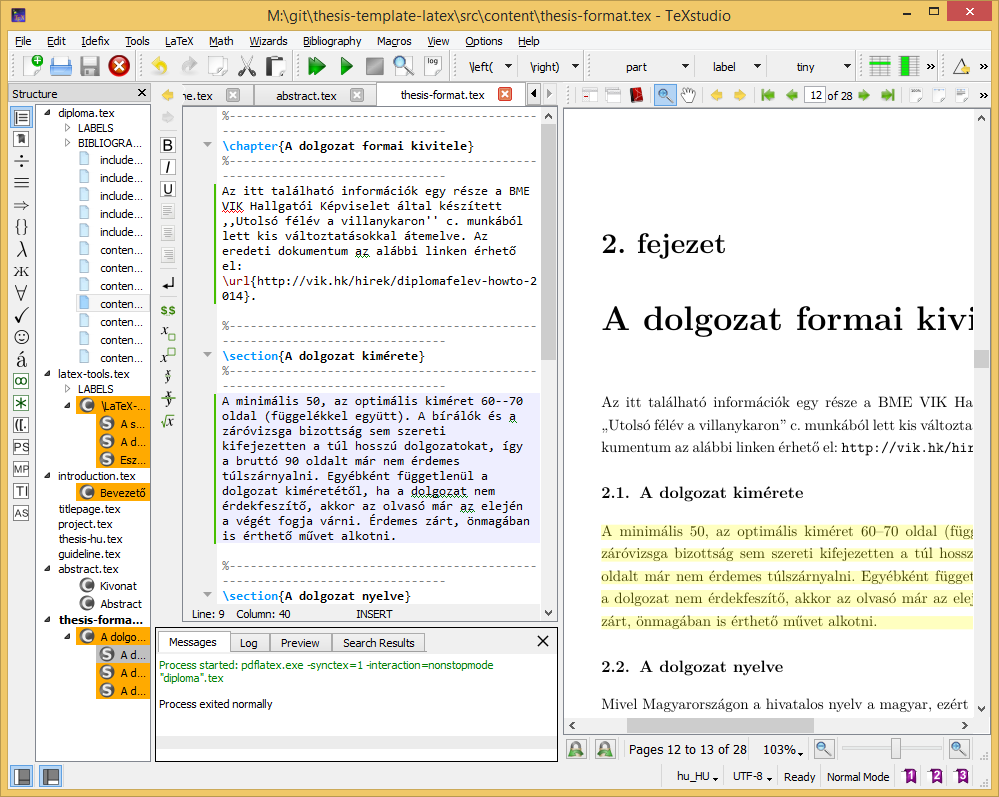
\includegraphics[width=150mm, keepaspectratio]{figures/TeXstudio.png}
\caption{A TeXstudio \LaTeX-szerkesztő.} 
\end{figure}
